% Options for packages loaded elsewhere
\PassOptionsToPackage{unicode}{hyperref}
\PassOptionsToPackage{hyphens}{url}
\PassOptionsToPackage{dvipsnames,svgnames,x11names}{xcolor}
%
\documentclass[
  letterpaper,
  DIV=11,
  numbers=noendperiod]{scrartcl}

\usepackage{amsmath,amssymb}
\usepackage{iftex}
\ifPDFTeX
  \usepackage[T1]{fontenc}
  \usepackage[utf8]{inputenc}
  \usepackage{textcomp} % provide euro and other symbols
\else % if luatex or xetex
  \usepackage{unicode-math}
  \defaultfontfeatures{Scale=MatchLowercase}
  \defaultfontfeatures[\rmfamily]{Ligatures=TeX,Scale=1}
\fi
\usepackage{lmodern}
\ifPDFTeX\else  
    % xetex/luatex font selection
\fi
% Use upquote if available, for straight quotes in verbatim environments
\IfFileExists{upquote.sty}{\usepackage{upquote}}{}
\IfFileExists{microtype.sty}{% use microtype if available
  \usepackage[]{microtype}
  \UseMicrotypeSet[protrusion]{basicmath} % disable protrusion for tt fonts
}{}
\makeatletter
\@ifundefined{KOMAClassName}{% if non-KOMA class
  \IfFileExists{parskip.sty}{%
    \usepackage{parskip}
  }{% else
    \setlength{\parindent}{0pt}
    \setlength{\parskip}{6pt plus 2pt minus 1pt}}
}{% if KOMA class
  \KOMAoptions{parskip=half}}
\makeatother
\usepackage{xcolor}
\setlength{\emergencystretch}{3em} % prevent overfull lines
\setcounter{secnumdepth}{5}
% Make \paragraph and \subparagraph free-standing
\makeatletter
\ifx\paragraph\undefined\else
  \let\oldparagraph\paragraph
  \renewcommand{\paragraph}{
    \@ifstar
      \xxxParagraphStar
      \xxxParagraphNoStar
  }
  \newcommand{\xxxParagraphStar}[1]{\oldparagraph*{#1}\mbox{}}
  \newcommand{\xxxParagraphNoStar}[1]{\oldparagraph{#1}\mbox{}}
\fi
\ifx\subparagraph\undefined\else
  \let\oldsubparagraph\subparagraph
  \renewcommand{\subparagraph}{
    \@ifstar
      \xxxSubParagraphStar
      \xxxSubParagraphNoStar
  }
  \newcommand{\xxxSubParagraphStar}[1]{\oldsubparagraph*{#1}\mbox{}}
  \newcommand{\xxxSubParagraphNoStar}[1]{\oldsubparagraph{#1}\mbox{}}
\fi
\makeatother


\providecommand{\tightlist}{%
  \setlength{\itemsep}{0pt}\setlength{\parskip}{0pt}}\usepackage{longtable,booktabs,array}
\usepackage{calc} % for calculating minipage widths
% Correct order of tables after \paragraph or \subparagraph
\usepackage{etoolbox}
\makeatletter
\patchcmd\longtable{\par}{\if@noskipsec\mbox{}\fi\par}{}{}
\makeatother
% Allow footnotes in longtable head/foot
\IfFileExists{footnotehyper.sty}{\usepackage{footnotehyper}}{\usepackage{footnote}}
\makesavenoteenv{longtable}
\usepackage{graphicx}
\makeatletter
\def\maxwidth{\ifdim\Gin@nat@width>\linewidth\linewidth\else\Gin@nat@width\fi}
\def\maxheight{\ifdim\Gin@nat@height>\textheight\textheight\else\Gin@nat@height\fi}
\makeatother
% Scale images if necessary, so that they will not overflow the page
% margins by default, and it is still possible to overwrite the defaults
% using explicit options in \includegraphics[width, height, ...]{}
\setkeys{Gin}{width=\maxwidth,height=\maxheight,keepaspectratio}
% Set default figure placement to htbp
\makeatletter
\def\fps@figure{htbp}
\makeatother

\KOMAoption{captions}{tableheading}
\makeatletter
\@ifpackageloaded{tcolorbox}{}{\usepackage[skins,breakable]{tcolorbox}}
\@ifpackageloaded{fontawesome5}{}{\usepackage{fontawesome5}}
\definecolor{quarto-callout-color}{HTML}{909090}
\definecolor{quarto-callout-note-color}{HTML}{0758E5}
\definecolor{quarto-callout-important-color}{HTML}{CC1914}
\definecolor{quarto-callout-warning-color}{HTML}{EB9113}
\definecolor{quarto-callout-tip-color}{HTML}{00A047}
\definecolor{quarto-callout-caution-color}{HTML}{FC5300}
\definecolor{quarto-callout-color-frame}{HTML}{acacac}
\definecolor{quarto-callout-note-color-frame}{HTML}{4582ec}
\definecolor{quarto-callout-important-color-frame}{HTML}{d9534f}
\definecolor{quarto-callout-warning-color-frame}{HTML}{f0ad4e}
\definecolor{quarto-callout-tip-color-frame}{HTML}{02b875}
\definecolor{quarto-callout-caution-color-frame}{HTML}{fd7e14}
\makeatother
\makeatletter
\@ifpackageloaded{caption}{}{\usepackage{caption}}
\AtBeginDocument{%
\ifdefined\contentsname
  \renewcommand*\contentsname{Table of contents}
\else
  \newcommand\contentsname{Table of contents}
\fi
\ifdefined\listfigurename
  \renewcommand*\listfigurename{List of Figures}
\else
  \newcommand\listfigurename{List of Figures}
\fi
\ifdefined\listtablename
  \renewcommand*\listtablename{List of Tables}
\else
  \newcommand\listtablename{List of Tables}
\fi
\ifdefined\figurename
  \renewcommand*\figurename{Figure}
\else
  \newcommand\figurename{Figure}
\fi
\ifdefined\tablename
  \renewcommand*\tablename{Table}
\else
  \newcommand\tablename{Table}
\fi
}
\@ifpackageloaded{float}{}{\usepackage{float}}
\floatstyle{ruled}
\@ifundefined{c@chapter}{\newfloat{codelisting}{h}{lop}}{\newfloat{codelisting}{h}{lop}[chapter]}
\floatname{codelisting}{Listing}
\newcommand*\listoflistings{\listof{codelisting}{List of Listings}}
\makeatother
\makeatletter
\makeatother
\makeatletter
\@ifpackageloaded{caption}{}{\usepackage{caption}}
\@ifpackageloaded{subcaption}{}{\usepackage{subcaption}}
\makeatother

\ifLuaTeX
  \usepackage{selnolig}  % disable illegal ligatures
\fi
\usepackage{bookmark}

\IfFileExists{xurl.sty}{\usepackage{xurl}}{} % add URL line breaks if available
\urlstyle{same} % disable monospaced font for URLs
\hypersetup{
  pdftitle={Module 3: Quantity and Operations},
  pdfauthor={Nathan Alexander, PhD},
  colorlinks=true,
  linkcolor={blue},
  filecolor={Maroon},
  citecolor={Blue},
  urlcolor={Blue},
  pdfcreator={LaTeX via pandoc}}


\title{Module 3: Quantity and Operations}
\usepackage{etoolbox}
\makeatletter
\providecommand{\subtitle}[1]{% add subtitle to \maketitle
  \apptocmd{\@title}{\par {\large #1 \par}}{}{}
}
\makeatother
\subtitle{EDUC 315 - Howard University}
\author{Nathan Alexander, PhD}
\date{}

\begin{document}
\maketitle

\renewcommand*\contentsname{Table of contents}
{
\hypersetup{linkcolor=}
\setcounter{tocdepth}{3}
\tableofcontents
}

Module: Quantity and Operations

\subsection{Module Overview}\label{module-overview}

This module explores the mathematical concepts focusing on quantity and
operations within the context of elementary mathematics. The module
covers the historical development of arithmetic operations, introduces
the Concrete-Representational-Abstract (CRA) approach to teaching
mathematics, delves into the properties of basic arithmetic operations,
and examines the relationships between different operations. By the end
of this module, you will have a comprehensive understanding of quantity
and operations to effectively deal with various mathematical
representations.

\section{Quantity and Operations}\label{quantity-and-operations}

\begin{tcolorbox}[enhanced jigsaw, rightrule=.15mm, toprule=.15mm, colbacktitle=quarto-callout-note-color!10!white, title={Quantity}, arc=.35mm, opacityback=0, left=2mm, toptitle=1mm, colback=white, breakable, coltitle=black, leftrule=.75mm, bottomtitle=1mm, titlerule=0mm, bottomrule=.15mm, opacitybacktitle=0.6, colframe=quarto-callout-note-color-frame]

A quantity is a property or characteristic that can be measured or
counted. In mathematics, it refers to an amount that can be expressed as
a number or a numerical value.

\end{tcolorbox}

Key points:

\begin{itemize}
\tightlist
\item
  Quantities can be discrete (countable) or continuous (measurable)
\item
  Quantities are often associated with units of measurement
\item
  Quantities form the basis for mathematical operations and comparisons
\end{itemize}

Examples:

\begin{itemize}
\tightlist
\item
  The number of apples in a basket (discrete quantity)
\item
  The volume of water in a container (continuous quantity)
\item
  The temperature of a room (measurable quantity)
\item
  The speed of a car (derived quantity)
\end{itemize}

\begin{center}\rule{0.5\linewidth}{0.5pt}\end{center}

\begin{tcolorbox}[enhanced jigsaw, rightrule=.15mm, toprule=.15mm, colbacktitle=quarto-callout-note-color!10!white, title={Operation}, arc=.35mm, opacityback=0, left=2mm, toptitle=1mm, colback=white, breakable, coltitle=black, leftrule=.75mm, bottomtitle=1mm, titlerule=0mm, bottomrule=.15mm, opacitybacktitle=0.6, colframe=quarto-callout-note-color-frame]

An operation is a mathematical process or action performed on one or
more quantities to produce a new quantity or result. It is a rule for
combining mathematical objects or values.

\end{tcolorbox}

\begin{itemize}
\tightlist
\item
  Operations transform quantities into new quantities
\item
  They follow specific rules and properties (e.g., commutative,
  associative)
\item
  Understanding operations is crucial for problem-solving and algebraic
  thinking
\end{itemize}

\begin{tcolorbox}[enhanced jigsaw, rightrule=.15mm, toprule=.15mm, colbacktitle=quarto-callout-tip-color!10!white, title=\textcolor{quarto-callout-tip-color}{\faLightbulb}\hspace{0.5em}{Addition (sum)}, arc=.35mm, opacityback=0, left=2mm, toptitle=1mm, colback=white, breakable, coltitle=black, leftrule=.75mm, bottomtitle=1mm, titlerule=0mm, bottomrule=.15mm, opacitybacktitle=0.6, colframe=quarto-callout-tip-color-frame]

Combining two or more quantities (e.g., 5 + 3 = 8)

\end{tcolorbox}

\begin{tcolorbox}[enhanced jigsaw, rightrule=.15mm, toprule=.15mm, colbacktitle=quarto-callout-tip-color!10!white, title=\textcolor{quarto-callout-tip-color}{\faLightbulb}\hspace{0.5em}{Subtraction (difference)}, arc=.35mm, opacityback=0, left=2mm, toptitle=1mm, colback=white, breakable, coltitle=black, leftrule=.75mm, bottomtitle=1mm, titlerule=0mm, bottomrule=.15mm, opacitybacktitle=0.6, colframe=quarto-callout-tip-color-frame]

Finding the difference between quantities (e.g., 10 - 4 = 6)

\end{tcolorbox}

\begin{tcolorbox}[enhanced jigsaw, rightrule=.15mm, toprule=.15mm, colbacktitle=quarto-callout-tip-color!10!white, title=\textcolor{quarto-callout-tip-color}{\faLightbulb}\hspace{0.5em}{Multiplication (product)}, arc=.35mm, opacityback=0, left=2mm, toptitle=1mm, colback=white, breakable, coltitle=black, leftrule=.75mm, bottomtitle=1mm, titlerule=0mm, bottomrule=.15mm, opacitybacktitle=0.6, colframe=quarto-callout-tip-color-frame]

Repeated addition or scaling (e.g., 3 × 4 = 12)

\end{tcolorbox}

\begin{tcolorbox}[enhanced jigsaw, rightrule=.15mm, toprule=.15mm, colbacktitle=quarto-callout-tip-color!10!white, title=\textcolor{quarto-callout-tip-color}{\faLightbulb}\hspace{0.5em}{Division (quotient)}, arc=.35mm, opacityback=0, left=2mm, toptitle=1mm, colback=white, breakable, coltitle=black, leftrule=.75mm, bottomtitle=1mm, titlerule=0mm, bottomrule=.15mm, opacitybacktitle=0.6, colframe=quarto-callout-tip-color-frame]

Distributing a quantity into equal parts (e.g., 15 ÷ 3 = 5)

\end{tcolorbox}

\begin{tcolorbox}[enhanced jigsaw, rightrule=.15mm, toprule=.15mm, colbacktitle=quarto-callout-tip-color!10!white, title=\textcolor{quarto-callout-tip-color}{\faLightbulb}\hspace{0.5em}{Exponentiation (exponent)}, arc=.35mm, opacityback=0, left=2mm, toptitle=1mm, colback=white, breakable, coltitle=black, leftrule=.75mm, bottomtitle=1mm, titlerule=0mm, bottomrule=.15mm, opacitybacktitle=0.6, colframe=quarto-callout-tip-color-frame]

Repeated multiplication (e.g., 2³ = 8)

\end{tcolorbox}

\begin{tcolorbox}[enhanced jigsaw, rightrule=.15mm, toprule=.15mm, colbacktitle=quarto-callout-tip-color!10!white, title=\textcolor{quarto-callout-tip-color}{\faLightbulb}\hspace{0.5em}{Root extraction (root)}, arc=.35mm, opacityback=0, left=2mm, toptitle=1mm, colback=white, breakable, coltitle=black, leftrule=.75mm, bottomtitle=1mm, titlerule=0mm, bottomrule=.15mm, opacitybacktitle=0.6, colframe=quarto-callout-tip-color-frame]

Inverse of exponentiation (e.g., \(\sqrt{16} = 4\))

\end{tcolorbox}

\subsection{Concrete-Representational-Abstract
(CRA)}\label{concrete-representational-abstract-cra}

The Concrete-Representational-Abstract (CRA) process is an instructional
approach in mathematics that helps students develop a deeper
understanding of mathematical concepts by progressing through three
stages:

\begin{enumerate}
\def\labelenumi{\arabic{enumi}.}
\tightlist
\item
  \textbf{Concrete} Stage:
\end{enumerate}

\begin{itemize}
\tightlist
\item
  Students use physical, hands-on objects to model mathematical concepts
\item
  Examples include base-10 blocks, counters, fraction bars, or algebra
  tiles
\item
  This stage allows students to manipulate tangible objects to solve
  problems
\end{itemize}

\begin{figure}[H]

{\centering 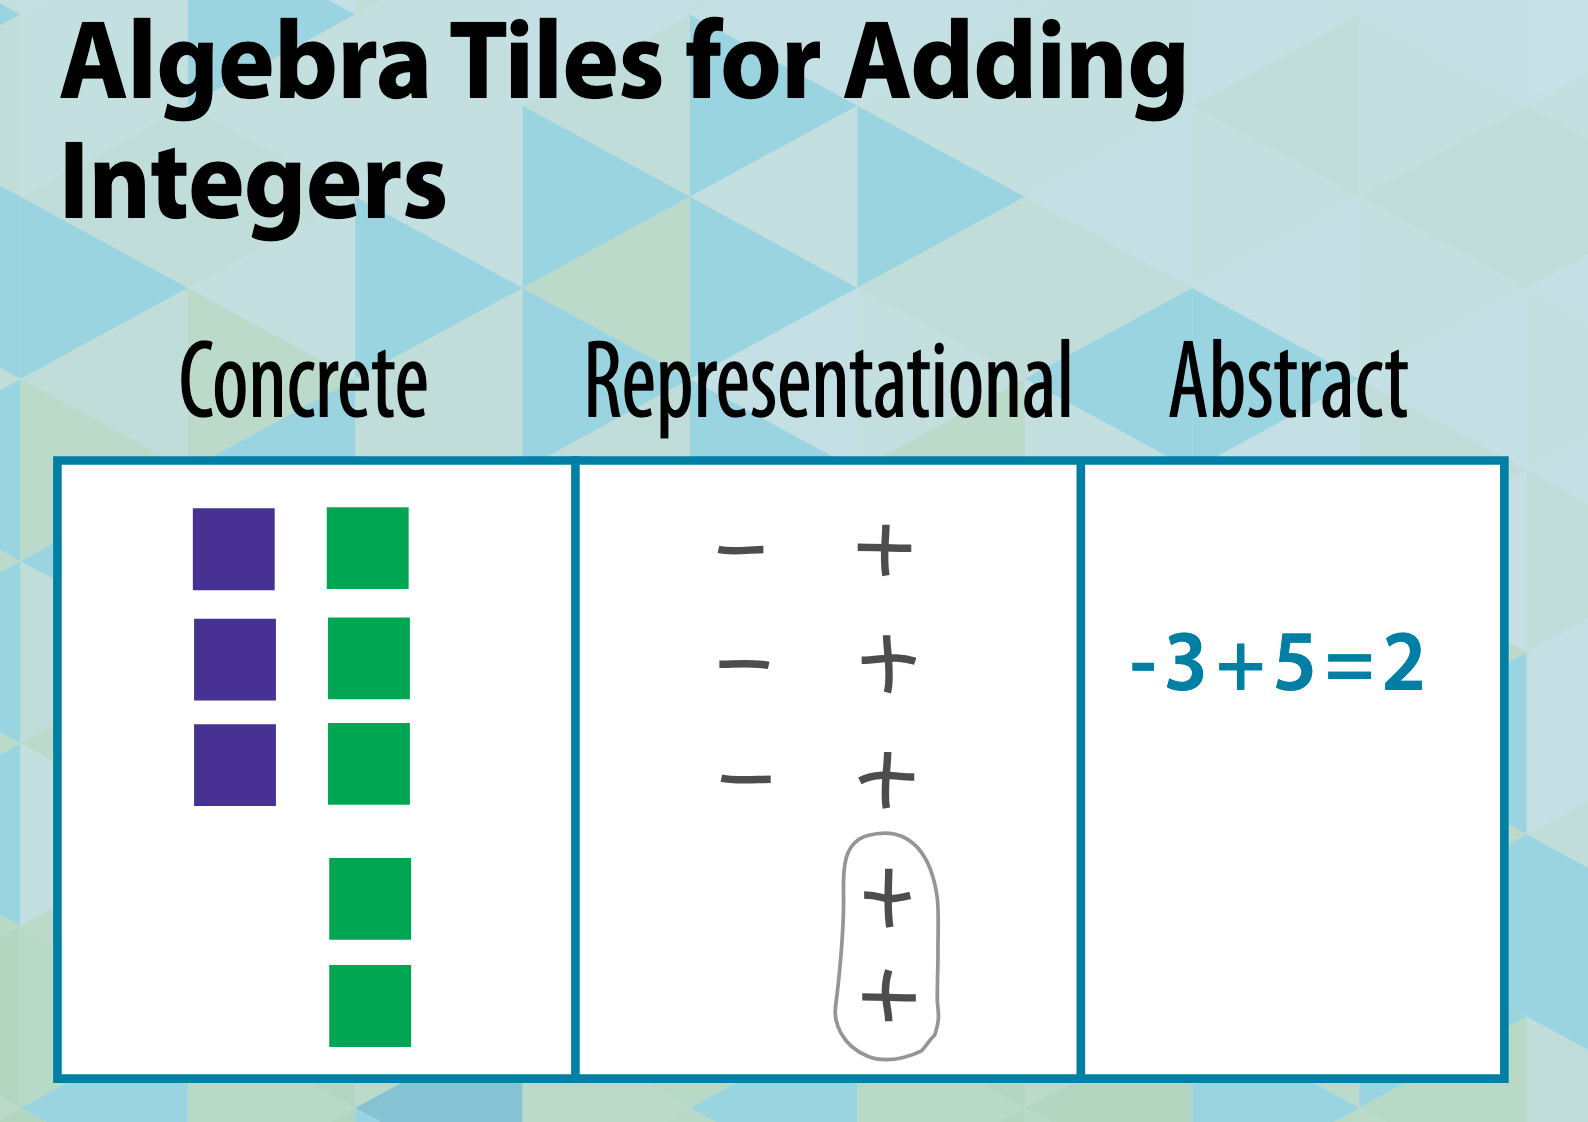
\includegraphics[width=0.8\textwidth,height=\textheight]{../img/mod03/cra-algebra-tiles-adding-integers.png}

}

\caption{Image from CRA methods by the Mathematics Initiative at
www.pattan.net}

\end{figure}%

\begin{enumerate}
\def\labelenumi{\arabic{enumi}.}
\setcounter{enumi}{1}
\tightlist
\item
  \textbf{Representational} (or Pictorial) Stage:
\end{enumerate}

\begin{itemize}
\tightlist
\item
  Students transition to using visual representations of the concrete
  objects
\item
  This may involve drawings, diagrams, or other pictorial models
\item
  Examples include number lines, bar models, or sketches of
  manipulatives
\end{itemize}

\begin{figure}[H]

{\centering 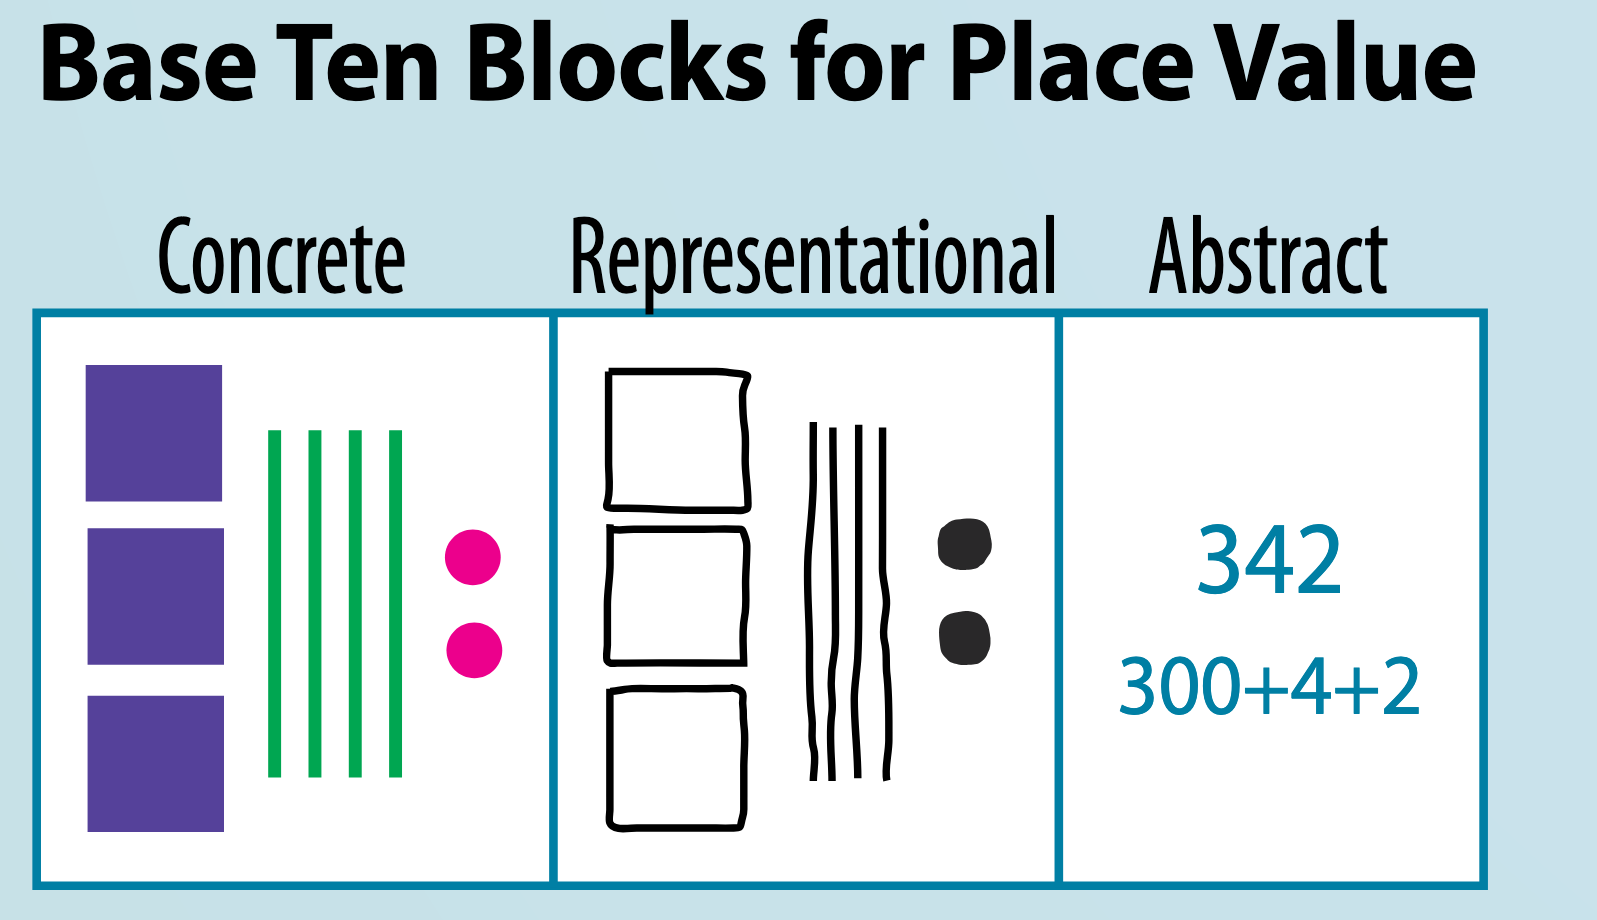
\includegraphics[width=0.8\textwidth,height=\textheight]{../img/mod03/cra-base-ten-blocks-place-value.png}

}

\caption{Image from CRA methods by the Mathematics Initiative at
www.pattan.net}

\end{figure}%

\begin{enumerate}
\def\labelenumi{\arabic{enumi}.}
\setcounter{enumi}{2}
\tightlist
\item
  \textbf{Abstract} Stage:
\end{enumerate}

\begin{itemize}
\tightlist
\item
  Students work with abstract symbols and notation
\item
  This includes numbers, variables, and mathematical symbols (+, -, x,
  ÷)
\item
  Students apply their understanding to solve problems using standard
  algorithms
\end{itemize}

\begin{figure}[H]

{\centering 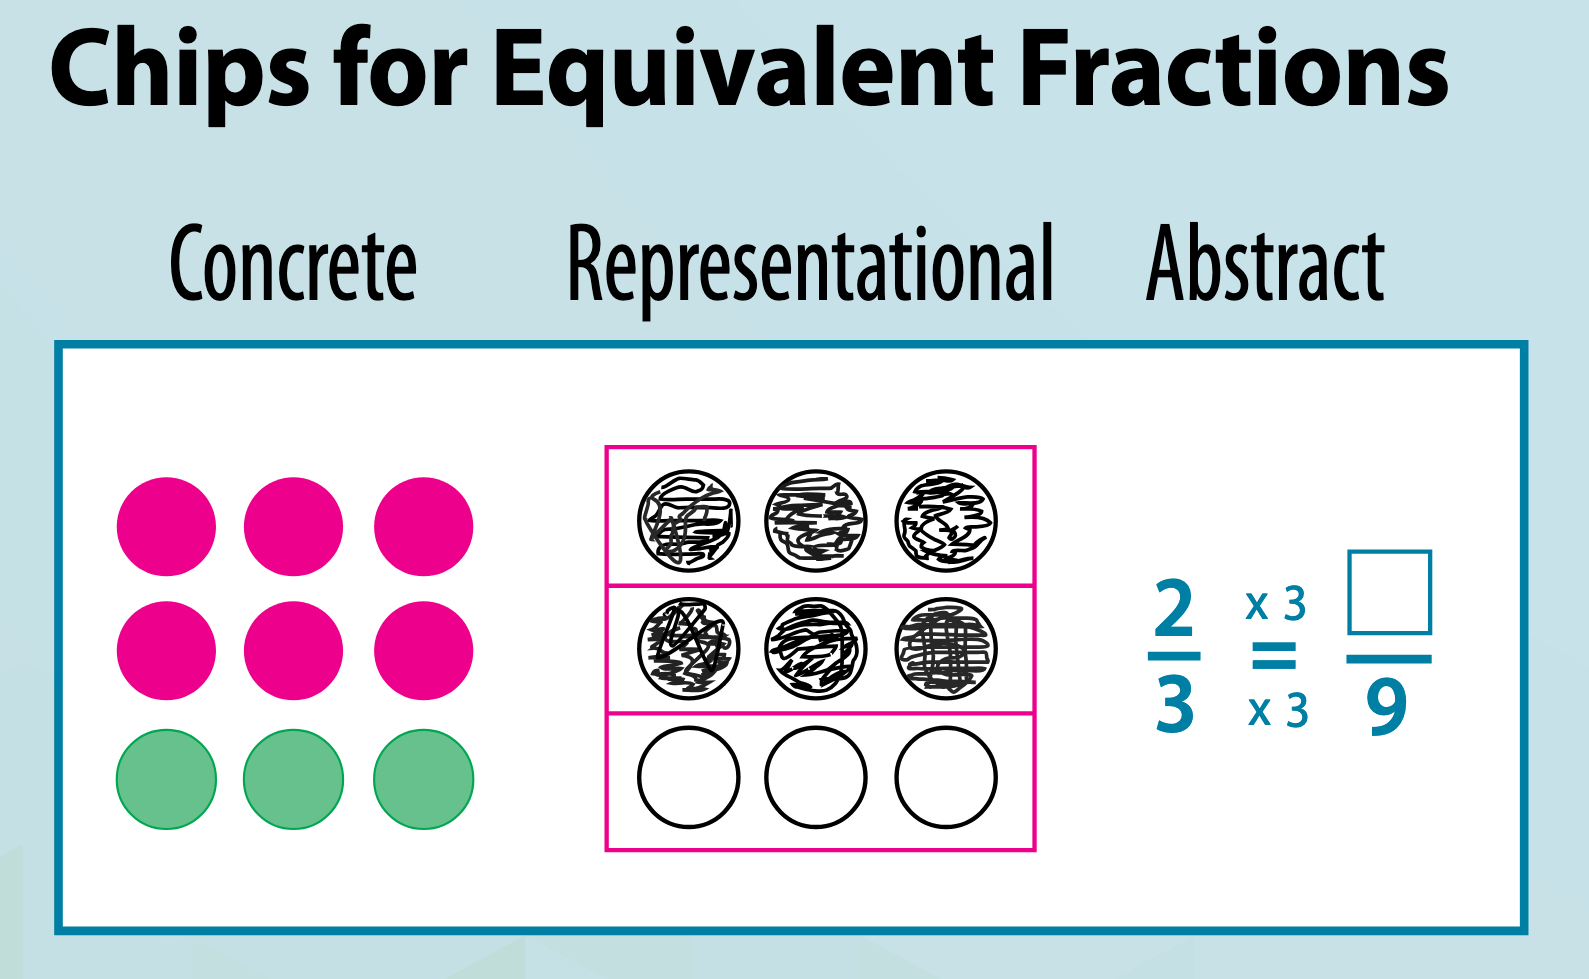
\includegraphics[width=0.8\textwidth,height=\textheight]{../img/mod03/cra-chips-equivalent-fractions.png}

}

\caption{Image from CRA methods by the Mathematics Initiative at
www.pattan.net}

\end{figure}%

The CRA approach deepens mathematical understanding and help students
internalize abstract concepts by first grounding them in concrete
experiences.

\begin{center}\rule{0.5\linewidth}{0.5pt}\end{center}

\section{Sum and Difference}\label{sum-and-difference}

\subsection{Algebra tiles}\label{algebra-tiles}

Depending on the grade of instruction, algebra tiles can be used as a
concrete way to express various operations, such as the sum and
difference.

\begin{figure}[H]

{\centering 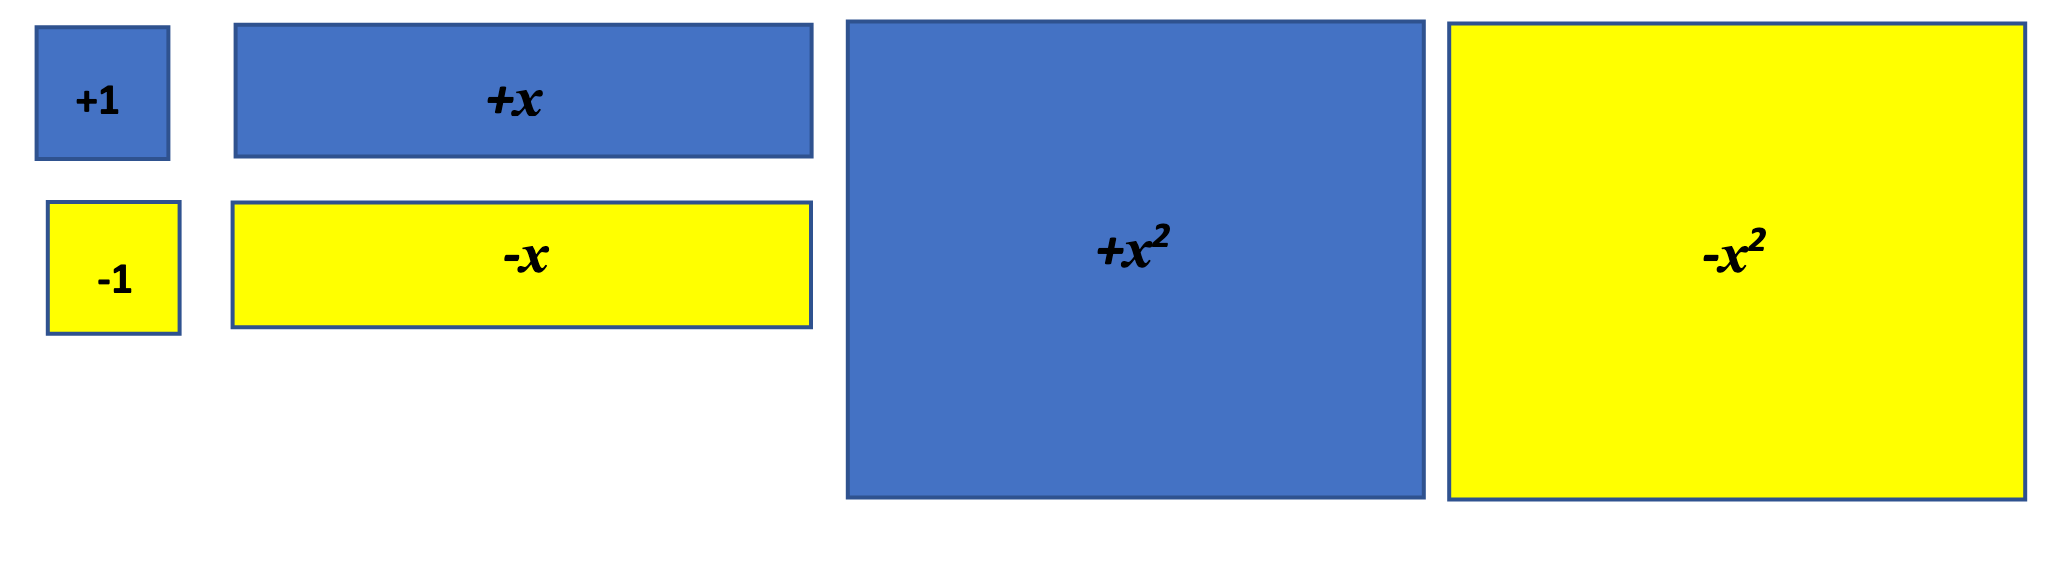
\includegraphics{../img/mod03/algebra-tile-0.png}

}

\caption{Introducing the tiles. From calculate.org.au}

\end{figure}%%
\begin{figure}[H]

{\centering 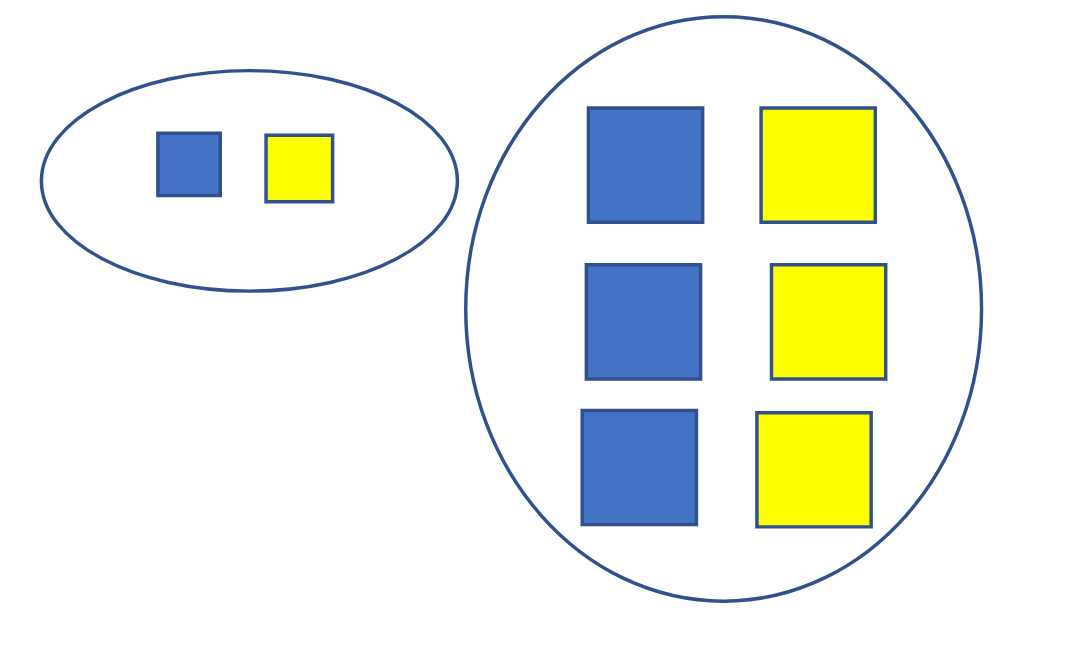
\includegraphics{../img/mod03/algebra-tile-1.png}

}

\caption{Zero-sum representation. From calculate.org.au}

\end{figure}%%
\begin{figure}[H]

{\centering 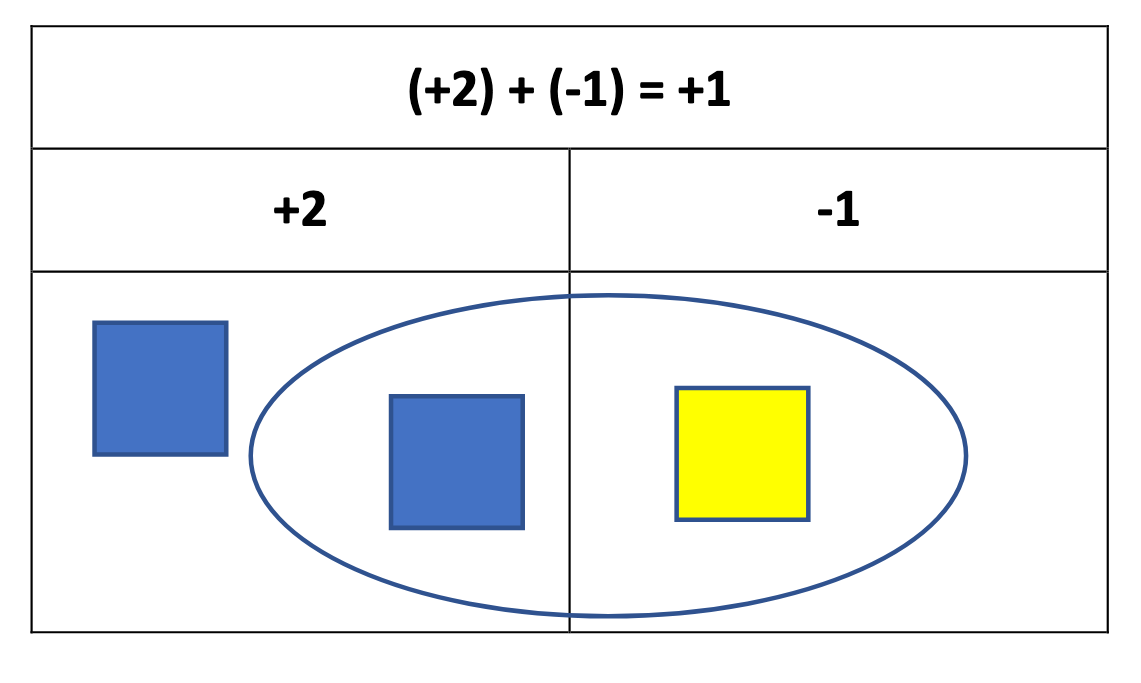
\includegraphics{../img/mod03/algebra-tile-2.png}

}

\caption{Modeling integers. From calculate.org.au}

\end{figure}%%
\begin{figure}[H]

{\centering 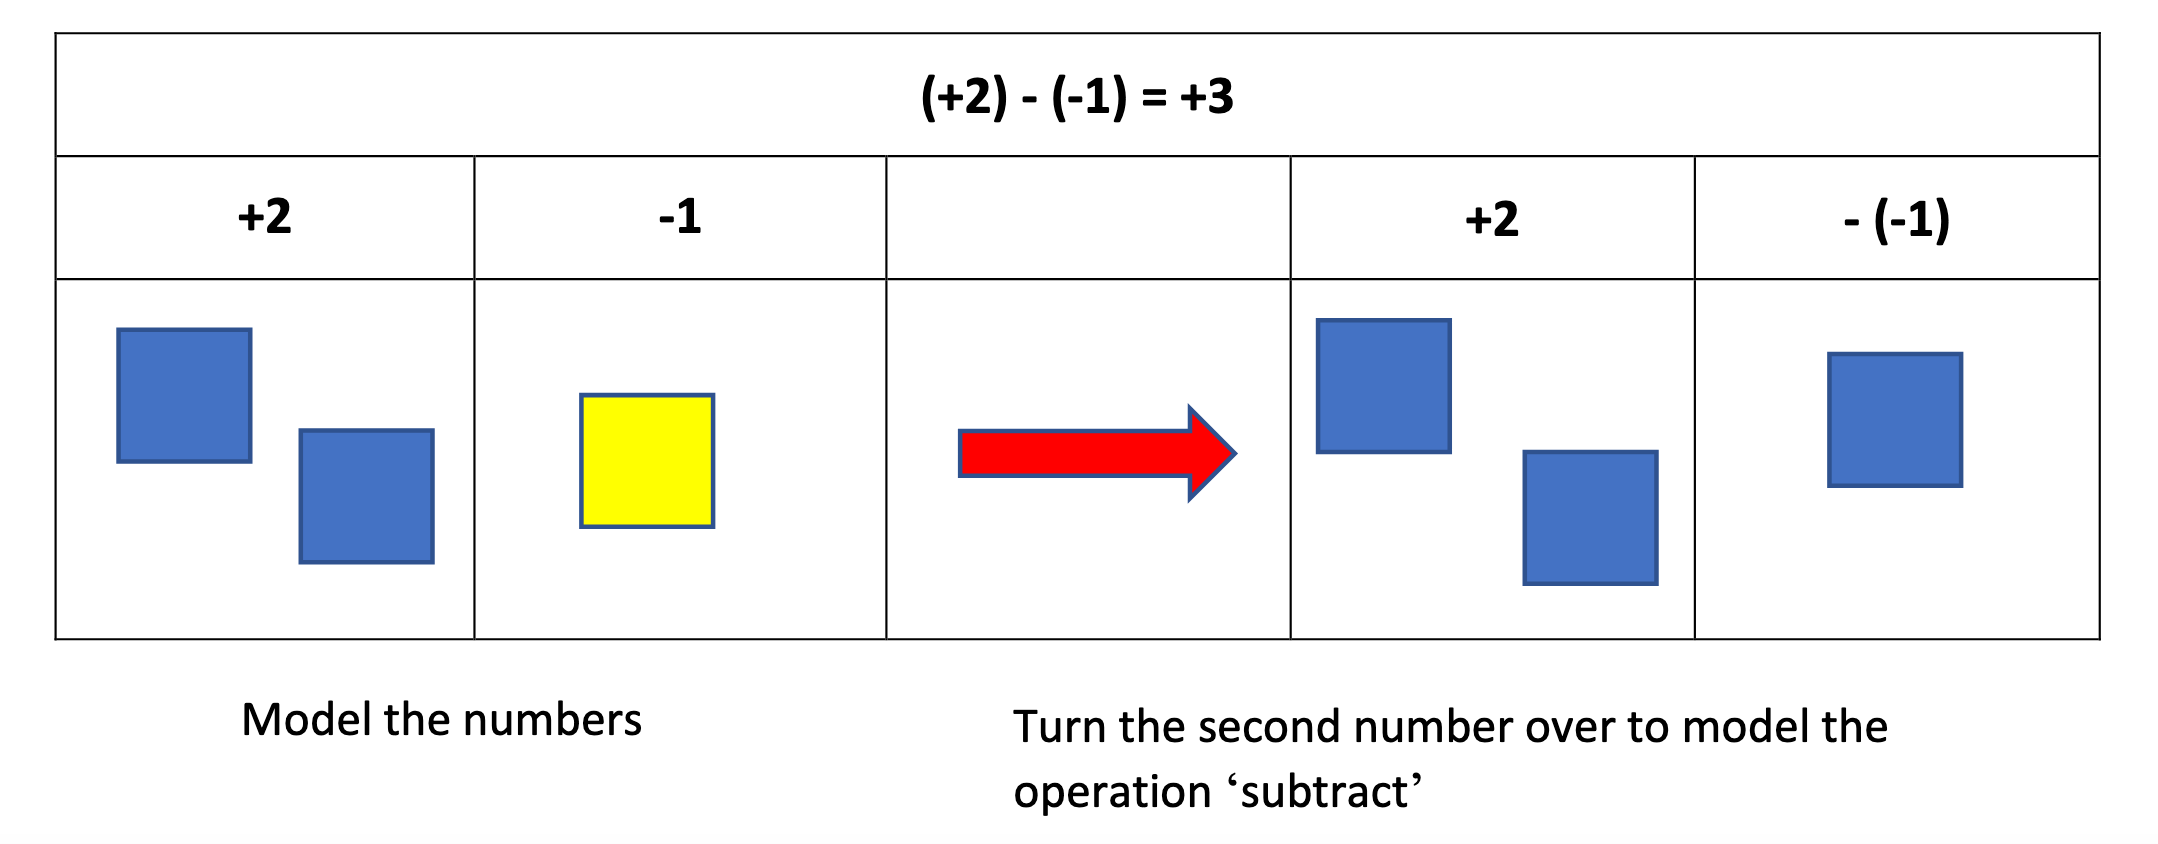
\includegraphics{../img/mod03/algebra-tile-3.png}

}

\caption{Addition and subtraction of integers. From calculate.org.au}

\end{figure}%

\begin{center}\rule{0.5\linewidth}{0.5pt}\end{center}

\section{Product and Quotient}\label{product-and-quotient}

Fraction tiles provide a great way to review and extend students'
understanding of the concepts of multiplication and division.

\begin{figure}[H]

{\centering 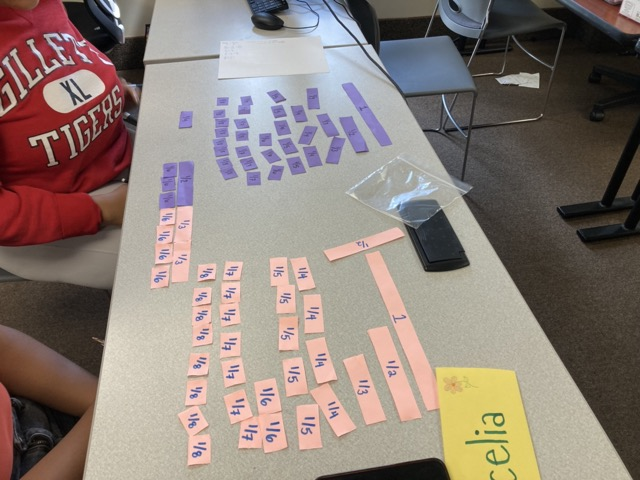
\includegraphics{../img/mod03/fraction-tiles-1.jpeg}

}

\caption{EDUC 315 fraction tiles}

\end{figure}%%
\begin{figure}[H]

{\centering 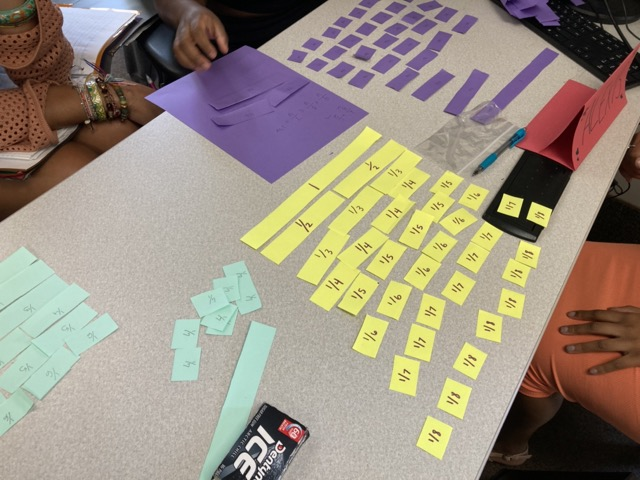
\includegraphics{../img/mod03/fraction-tiles-2.jpeg}

}

\caption{EDUC 315 fraction tiles}

\end{figure}%

\subsubsection{Assessing multiple
skills}\label{assessing-multiple-skills}

Multiplication (product) with fractions (quotients)

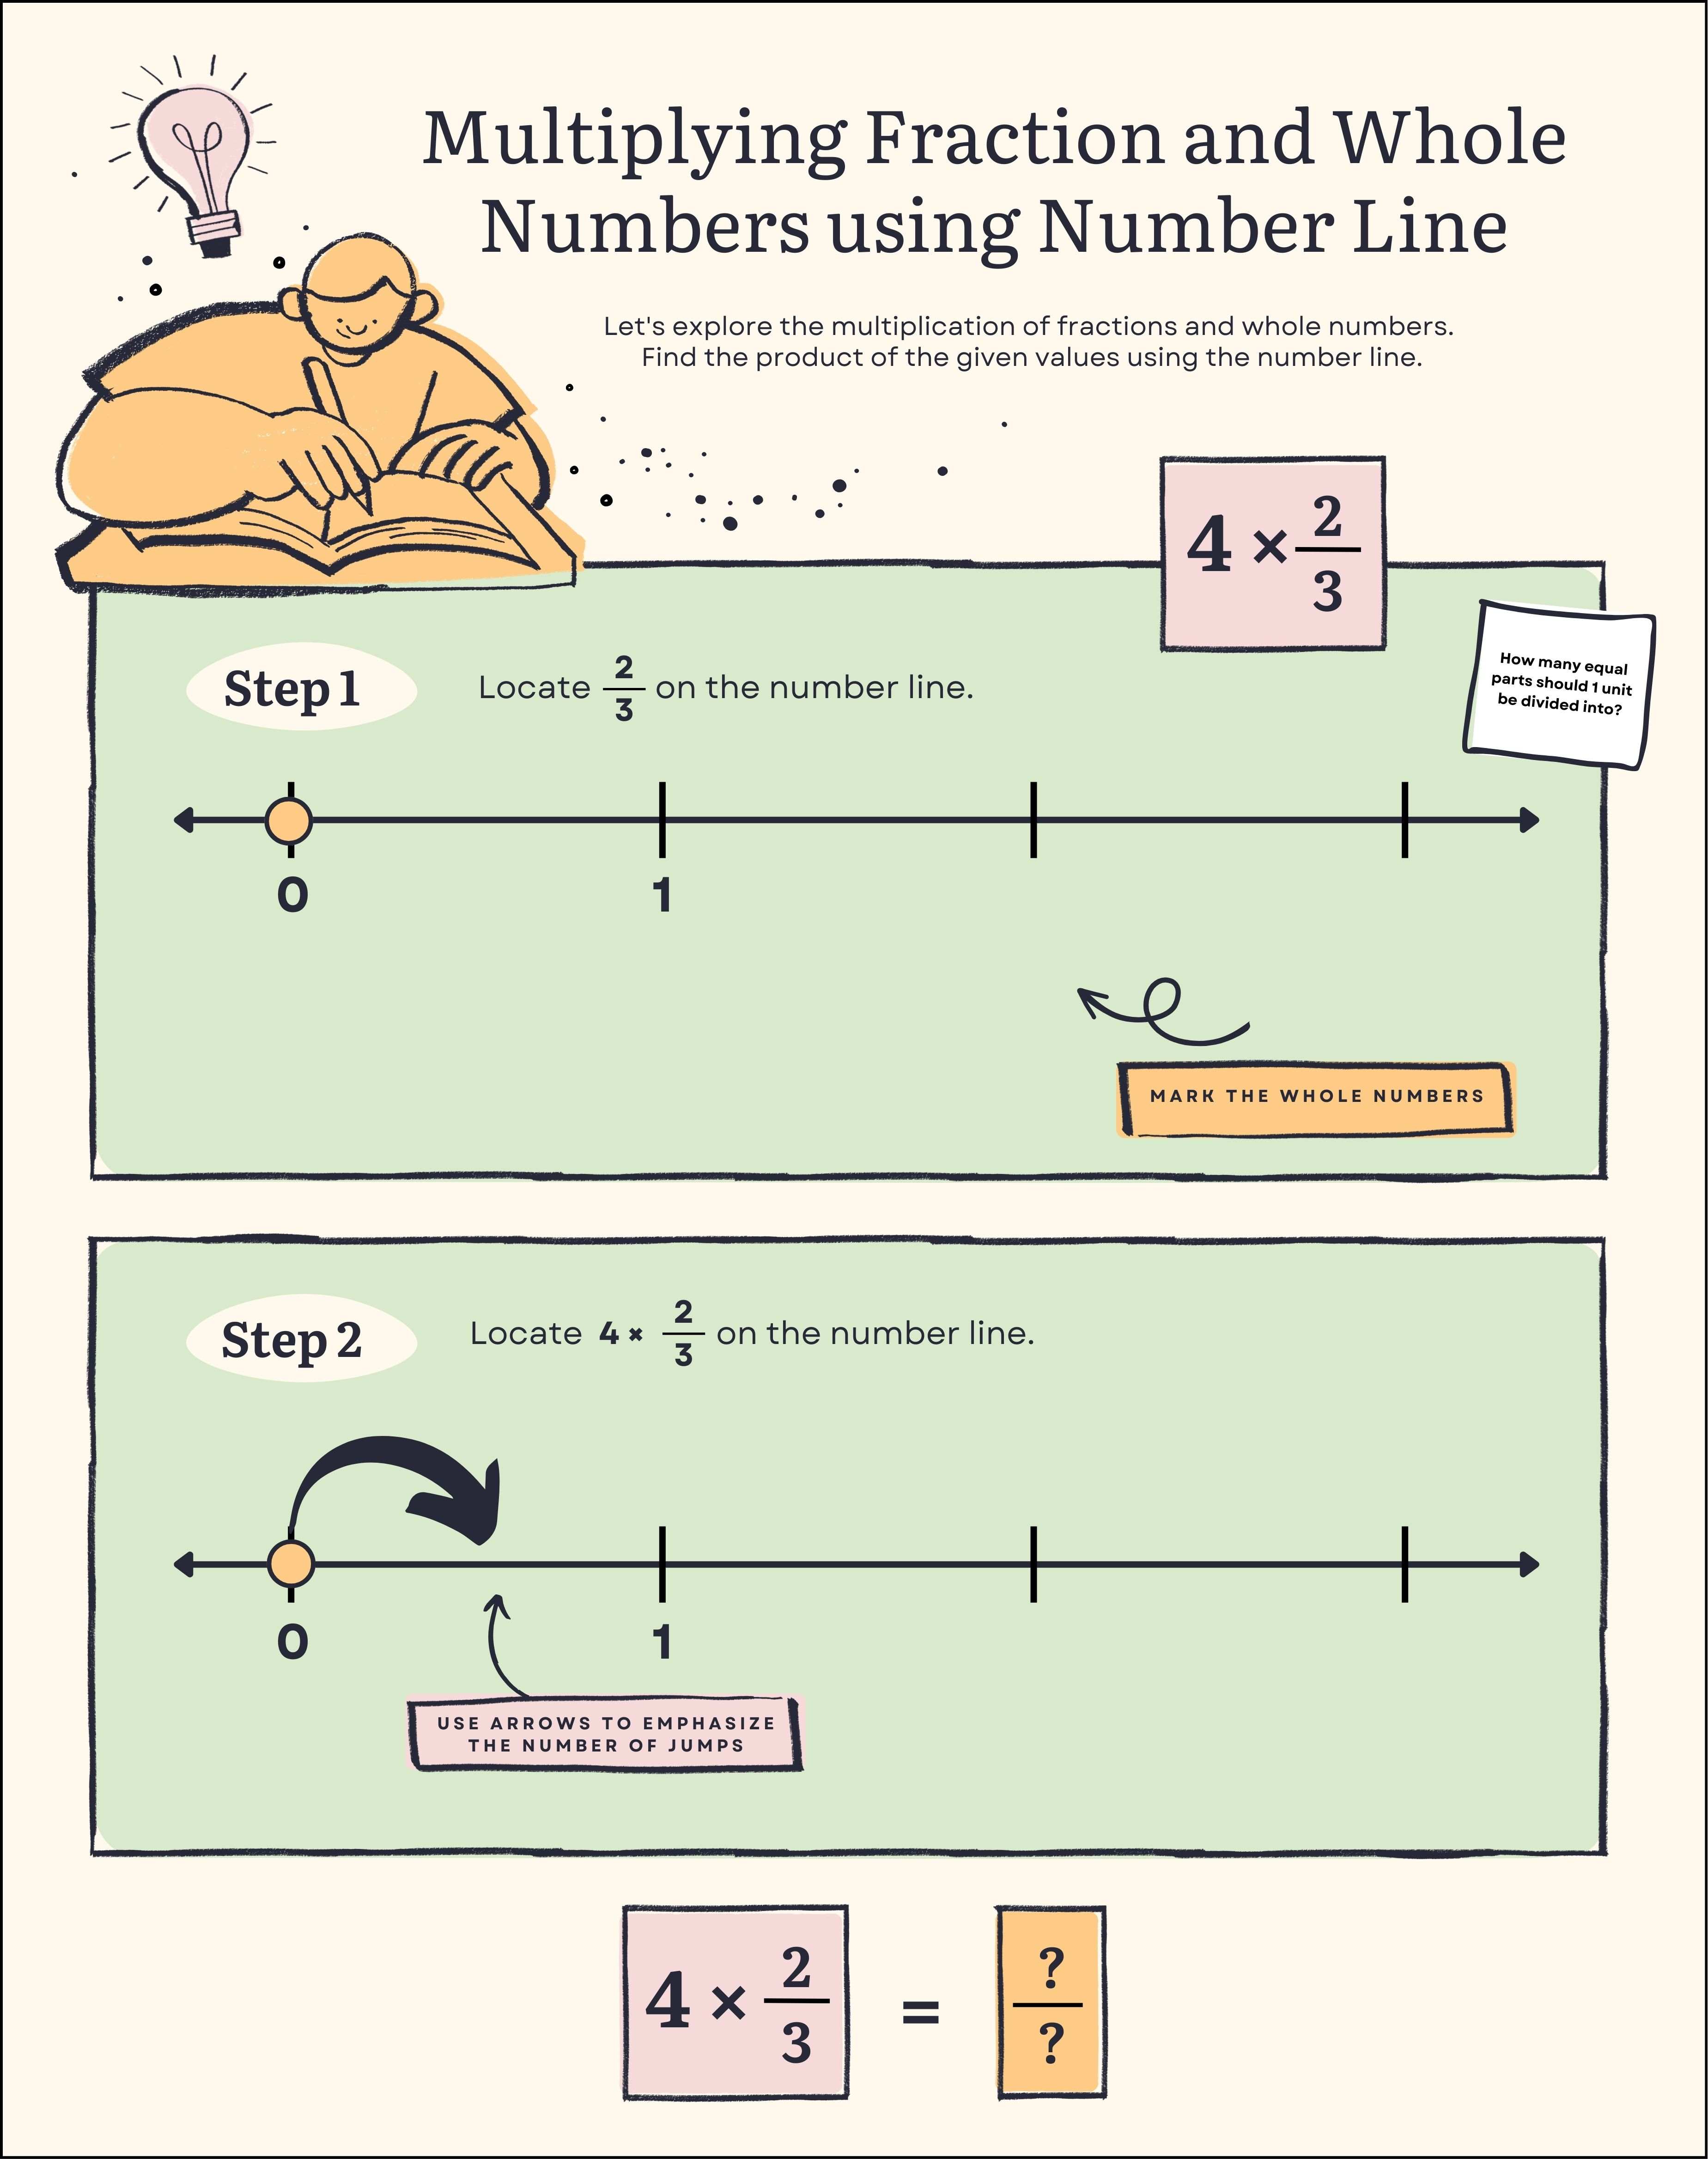
\includegraphics{../img/mod03/multiplying-fractions.jpg}

\begin{center}\rule{0.5\linewidth}{0.5pt}\end{center}

\section{Exponents and Roots}\label{exponents-and-roots}

There are many ways to teach exponents and roots:

\subsection{Teaching Exponents}\label{teaching-exponents}

\textbf{Pattern Blocks}

Pattern blocks can be used to visually demonstrate exponents. For
example:

\begin{itemize}
\tightlist
\item
  Use one triangle to represent \(1 \times 1\)
\item
  Four triangles together represent \(2 \times 2\)
\item
  Nine triangles together represent \(3 \times 3\)
\end{itemize}

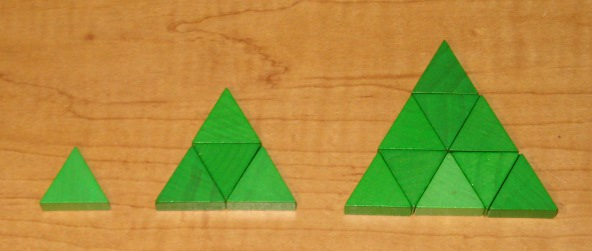
\includegraphics{../img/mod03/pattern-blocks.jpg}

Draw the pattern for \(4 \times 4\) and \(5 \times 5\).

These patterns helps students visualize the quantity of exponents but we
want to also show them representations of exponents as repeated
multiplication; we can use base-ten blocks to extend their
understanding.

\textbf{Base Ten Blocks}

Base ten blocks work well for teaching powers of 10:

\begin{itemize}
\tightlist
\item
  A unit cube represents \(10^0 = (1)\)
\item
  A rod represents \(10^1 = 10 = (10)\)
\item
  A flat represents \(10^2 = 10 x 10 = (100)\)
\item
  A large cube represents \(10^3 = 10 x 10 x 10 = (1000)\)
\end{itemize}

\textbf{Grid Paper}

Grid paper allows students to draw squares and rectangles to represent
exponents:

\begin{itemize}
\tightlist
\item
  A \(2 x 2\) square represents \(2^2\)
\item
  A \(3 x 3\) square represents \(3^2\)
\item
  A \(2 x 2 x 2\) cube represents \(2^3\)
\end{itemize}


\includegraphics{../img/mod03/grid-paper.jpg}

Draw the figures representing \(3^3\) and \(4^2\).

\subsection{Teaching Roots}\label{teaching-roots}

\textbf{Algebra Tiles}

Algebra tiles are also good for teaching square roots:

\begin{itemize}
\tightlist
\item
  Use the square tiles to build perfect square numbers (1, 4, 9, 16,
  etc.)
\item
  The side length of the square represents the square root
\end{itemize}

For example, a \(3x3\) square of tiles has an area of \(9\), so the
square root of \(9\) is \(3\).

\textbf{Grid Paper}

Grid paper can be used to estimate non-perfect square roots:

\begin{itemize}
\tightlist
\item
  Draw a square with the given area (e.g.~17)
\item
  Count the side length to estimate the square root
\item
  Refine by adding partial squares
\end{itemize}

This provides a visual model for estimating irrational square roots.

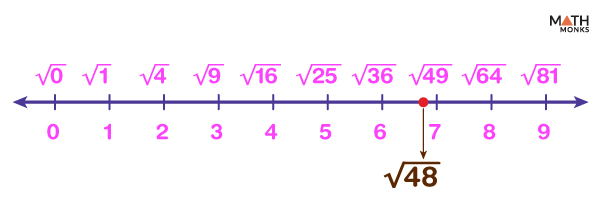
\includegraphics{../img/mod03/square-root-number-line.jpg}

\textbf{Number Lines}

Use a number line to place square roots between perfect squares:

\begin{itemize}
\tightlist
\item
  Mark perfect squares (1, 4, 9, 16, 25, etc.)
\item
  Estimate locations of other square roots between them
\end{itemize}

This helps students understand square roots as numbers between integers.

We can use manipulatives to build conceptual understanding before moving
to procedures. Allow students to explore and discover patterns through
hands-on activities. Gradually connect the concrete models to symbolic
notation as students gain understanding.

\begin{center}\rule{0.5\linewidth}{0.5pt}\end{center}

\section{STEM figures and history}\label{stem-figures-and-history}

Incorporating history into your mathematics lessons provide an
opportunity for interdisciplinary learning, and it encourages students
to see mathematics in action through real-world examples.

\subsection{Ancestral mathematics}\label{ancestral-mathematics}

\begin{figure}[H]

{\centering 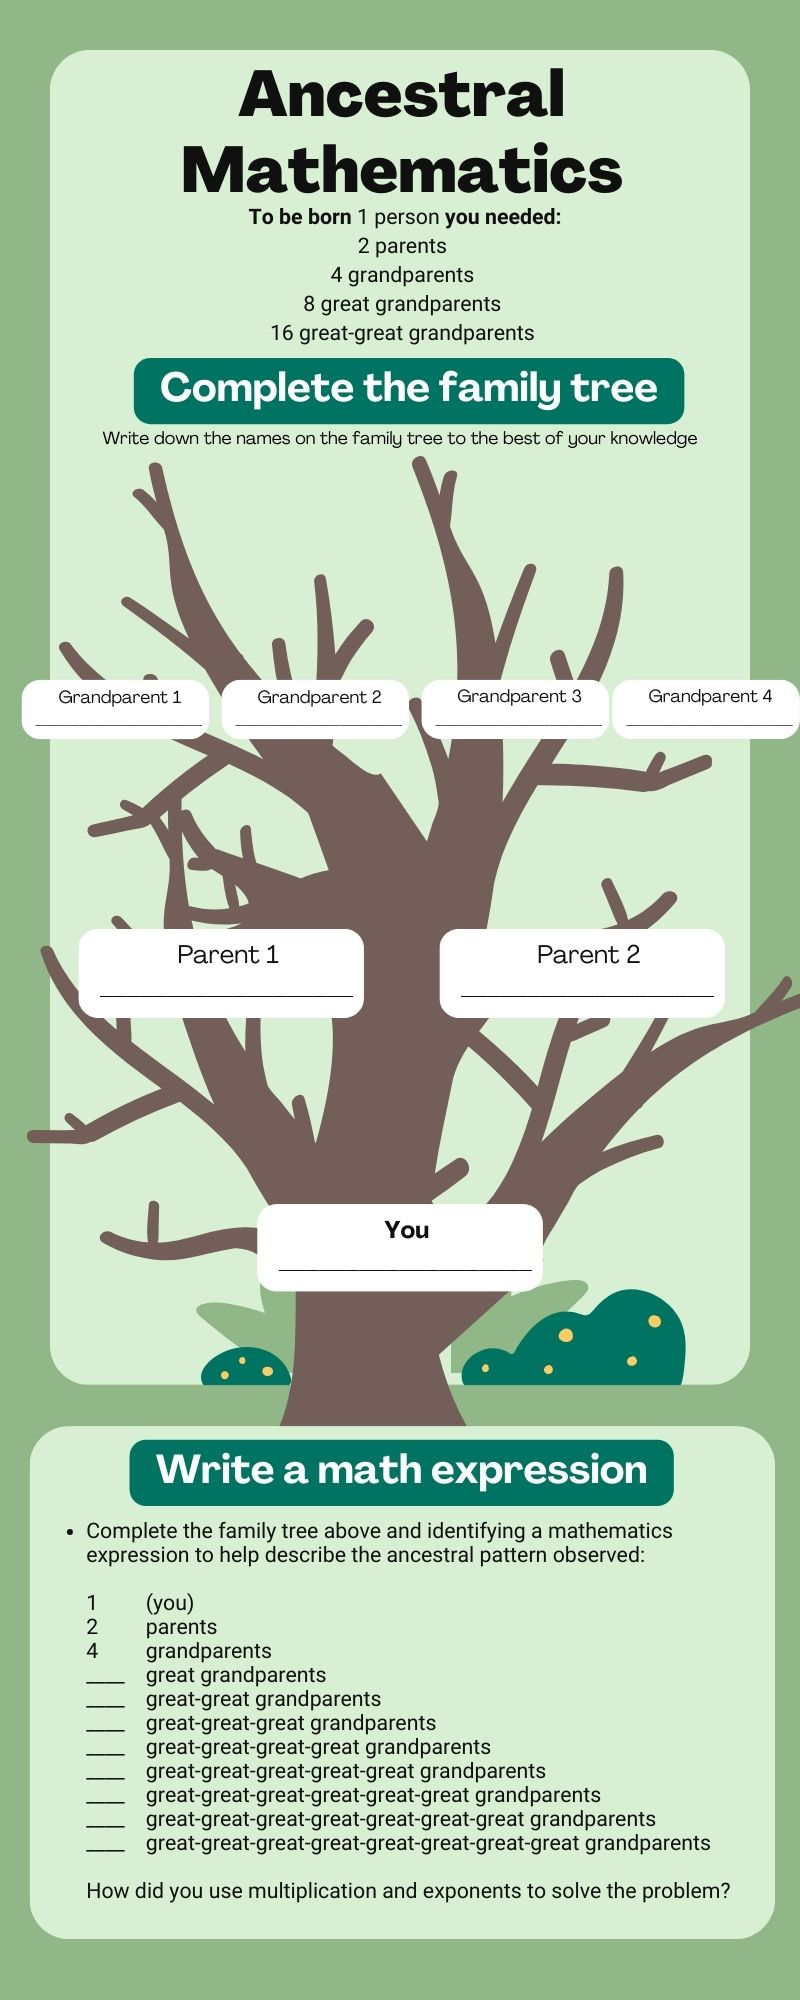
\includegraphics[width=0.5\textwidth,height=\textheight]{../img/mod03/ancestral-mathematics.jpg}

}

\caption{Ancestral mathematics activity by Dr.~Nathan Alexander. Adapted
from `Ancestral Mathematics' meme.}

\end{figure}%

Using the image above as a sample, outline an \emph{Ancestral
Mathematics} class activity and create or modify the worksheet to follow
along with your activity.

\subsection{Historical STEM Figures}\label{historical-stem-figures}

This module closes with the identification of a historical figure in
STEM.

\subsubsection{Objective}\label{objective}

Research a historical STEM figure and create engaging content to
showcase their contributions. The historical figure should showcase the
growing diversity of a host of identities, cultures, and backgrounds
represented in STEM.

\subsubsection{Procedures}\label{procedures}

\begin{itemize}
\item
  \emph{Museum visit} (75 minutes): Smithsonian Museum exhibit. Please
  take notes on interesting STEM figures and exhibits.
\item
  \emph{Figure selection and background research}: Choose a historical
  STEM figure based on museum inspiration. Conduct additional research
  using archival resources and online databases.
\item
  \emph{Content creation}: Students create content about their chosen
  figure in one of the following formats: Detailed video presentation
  (e.g., Tiktoc), Visual infographic (e.g., Canva), Interactive digital
  timeline, Podcast-like episode, Digital exhibit
\item
  \emph{Peer review}: Students your work with classmates for feedback.
  Make final adjustments based on peer feedback.
\item
  \emph{Presentation} (5 minutes): Develop a 5-minute presentation in
  the style that you would present it to your student. Present finished
  content to the class as if you were in front of your future students.
\end{itemize}

\begin{figure}[H]

{\centering 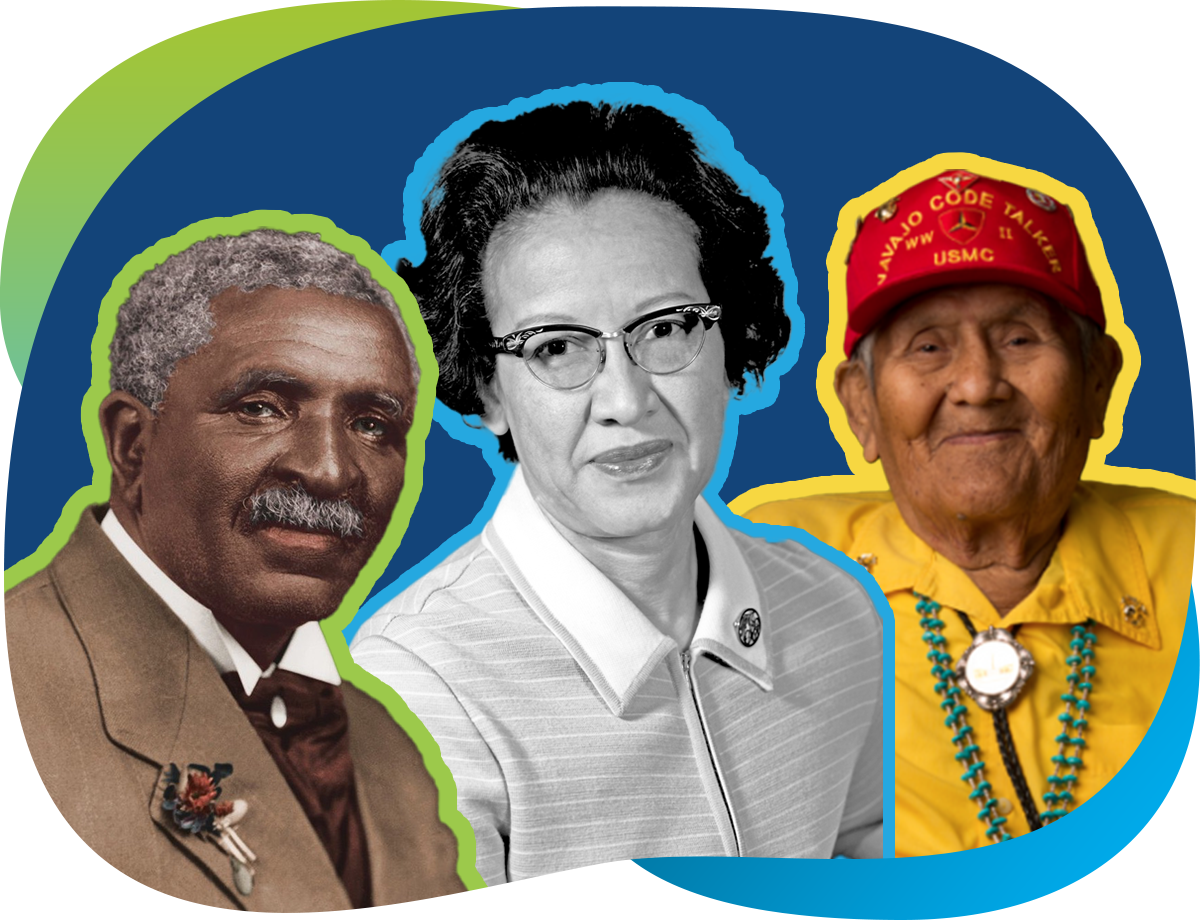
\includegraphics{../img/mod03/historical-figures.png}

}

\caption{Image from
\href{https://www.rif.org/literacy-central/sustainable-futures/careers-in-stem}{rif.org}}

\end{figure}%




\end{document}
